% One State, Many Forward-Maximal Futures
% Note for a philosophy-of-science venue (European Journal for Philosophy of
% Science): plain article class, 12pt, single column, numbered theorem
% environments.
%
% ANONYMISED FOR BLIND REVIEW. The author block, affiliation, postal address
% and e-mail address have been removed; restore them before publication.
%
% Build:  pdflatex one-state-many-futures  (twice, for cross-references)
% The figure needs figure-branches.tex, produced by make_figure_data.py.

\documentclass[12pt]{article}

\usepackage{lmodern}          % scalable Type 1 faces; microtype needs these
\usepackage[T1]{fontenc}
\usepackage[utf8]{inputenc}
\usepackage{amsmath, amssymb, amsthm}
\usepackage{mathtools}
\usepackage[margin=1.15in]{geometry}
\usepackage{microtype}
\usepackage{pgfplots}
\pgfplotsset{compat=1.18}
\usepackage[hidelinks]{hyperref}

\theoremstyle{plain}
\newtheorem{theorem}{Theorem}
\newtheorem{lemma}[theorem]{Lemma}
\newtheorem{proposition}[theorem]{Proposition}

\theoremstyle{definition}
\newtheorem{definition}[theorem]{Definition}
\newtheorem{example}[theorem]{Example}

\theoremstyle{remark}
\newtheorem{remark}[theorem]{Remark}

\newcommand{\R}{\mathbb{R}}
\newcommand{\cont}{\mathfrak{c}}
\newcommand{\Hglob}{\mathcal{H}^{+}_{\mathrm{glob}}}
\newcommand{\Hmax}{\mathcal{H}^{+}_{\max}}
\DeclareMathOperator{\sgn}{sgn}

\title{One State, Many Forward-Maximal Futures}
% Author block removed for blind review; restore before publication.
\author{}
\date{}

\begin{document}
\maketitle

\begin{abstract}
\noindent
For the initial-value problem $\dot x = f(x)$, $x(0)=0$ with $f$ continuous,
$f(0)=0$ and $f>0$ off the origin, the structure of the solution set is
classical: it was characterised by Wallach \cite{Wallach} in 1948 and treated in
general form by Binding \cite{Binding} in 1979. This note takes one concrete
member of that class, $f(x)=|x|^{2/3}+x^{2}$, and works it out completely.

The example has exactly one solution defined on all of $[0,\infty)$, namely
$x\equiv 0$, and continuum-many solutions that admit no forward extension: for
each waiting time $T\ge 0$ there is a solution that rests at the origin until
$T$, departs, and reaches $+\infty$ at $T+T_{*}$, where the escape time
$T_{*}<\infty$ is the same for every branch and is evaluated in closed form
below. Two independent mechanisms produce the two counts. Convergence of
$\int_{0}^{1}dx/f$ permits a continuum of waiting-time departures, which is what
makes the second count $\cont$; convergence of $\int_{1}^{\infty}dx/f$ forces
every non-trivial branch to reach $+\infty$ in finite time and so to fail to be
global, which is what leaves the first count at $1$. Neither mechanism alone
separates them.

The distinction this illustrates --- between uniqueness among globally defined
solutions and uniqueness among solutions that merely cannot be extended
forward --- is not introduced here either. It is discussed for general relativity by Earman
\cite{Earman}, Smeenk and W\"uthrich \cite{SmeenkWuthrich} and Doboszewski
\cite{Doboszewski}, for Newtonian blow-up by Wilson \cite{Wilson}, and within a
broader formulation of indeterminism by Azhar and Namjoo \cite{AzharNamjoo}.
What is offered here is an explicit worked example in which every quantity is
available in closed form, together with one proposition
(Proposition~\ref{prop:locality}) locating where each of the two uniqueness
verdicts is determined. \textbf{The example does not by itself establish that
any physical theory is indeterministic.} What it shows is that a uniqueness
verdict depends on which class of solutions is quantified over;
Section~\ref{sec:determinism} sets out the competing readings and adjudicates
between none of them.
\end{abstract}

%------------------------------------------------------------------
\section{Introduction}\label{sec:intro}

Here is a question with a less obvious answer than it looks.

\begin{quote}
\emph{If an initial state admits exactly one solution that exists for all future
times, does it follow that the state has a unique possible future history?}
\end{quote}

Not necessarily --- not if histories are taken to be solutions that cannot be
extended to any later time, rather than solutions defined at every future time. The
two classes can differ, and where they do, the uniqueness verdict can differ
with them. That distinction is the subject of this note; we claim no priority
for it, nor for the mathematics on which it rests.

We use \emph{history} throughout for a solution regarded as a candidate physical
evolution. Nothing in Sections~\ref{sec:example}--\ref{sec:senses} depends on
that identification; Section~\ref{sec:determinism} is where it does work, and
says so.

The mathematics is classical. For scalar autonomous equations the solution set
through an equilibrium was characterised by Wallach \cite{Wallach} in 1948, and
the general theory --- the exact conditions for departure from an equilibrium,
for escape to infinity in finite time, and for the structure of the solution set
--- is given by Binding \cite{Binding}. The conceptual point is also familiar.
In general relativity the maximal globally hyperbolic development of initial
data is unique while extensions past a Cauchy horizon are not, and whether to
restrict attention to the well-behaved class is a live question rather than a
settled one \cite{Earman, SmeenkWuthrich}. In Newtonian mechanics Wilson
\cite{Wilson} argues that failures of global existence are descriptive gaps
rather than failures of determinism, in explicit opposition to Earman and
Norton. Azhar and Namjoo \cite{AzharNamjoo} argue that a uniqueness-based
criterion misses the sense in which a terminating history is itself a failure of
determination.

What follows is therefore expository. Its purpose is to put the distinction into
a small explicit example and work it out in full: a single scalar equation,
elementary integrals, a blow-up time in closed form, an explicit solution
family. No general relativity, no $N$-body mechanics, no partial differential
equations, no geometry.

%------------------------------------------------------------------
\section{The example}\label{sec:example}

Throughout we study
\begin{equation}\label{eq:ivp}
  \dot x = f(x), \qquad x(0)=0,
\end{equation}
for a continuous $f\colon\R\to\R$.

\begin{definition}\label{def:solution}
A \emph{solution} of \eqref{eq:ivp} is a differentiable function $x\colon I\to\R$
on an interval $I\subseteq[0,\infty)$ with non-empty interior and $\min I = 0$,
satisfying $\dot x(t)=f(x(t))$ throughout, with one-sided derivatives at any
endpoint belonging to $I$.
\end{definition}

We work forward from $0$ until Appendix~\ref{app:twosided}. The standing
hypotheses are
\begin{enumerate}
  \item[(H1)] $f$ is continuous, $f(0)=0$, and $f(x)>0$ for $x\ne 0$;
  \item[(H2)] $\displaystyle\int_{0}^{1}\frac{dx}{f(x)}<\infty$;
  \item[(H3)] $\displaystyle\int_{1}^{\infty}\frac{dx}{f(x)}<\infty$.
\end{enumerate}

The example is
\[
  \boxed{\,f(x)=|x|^{2/3}+x^{2}.\,}
\]

Four properties matter, and all four are elementary.

\begin{lemma}\label{lem:properties}
For $f(x)=|x|^{2/3}+x^{2}$:
\begin{enumerate}
  \item[(i)] \textup{(H1)} holds.
  \item[(ii)] $f$ is not locally Lipschitz at the origin, but is $C^{1}$ on
        $\R\setminus\{0\}$, so the failure sits at exactly one point.
  \item[(iii)] The substitution $x=u^{3}$ gives
        $\dfrac{dx}{x^{2/3}+x^{2}}=\dfrac{3\,du}{1+u^{4}}$ for $x>0$.
  \item[(iv)] \textup{(H2)} and \textup{(H3)} both hold.
\end{enumerate}
\end{lemma}

\begin{proof}
(i) $|x|^{2/3}$ is the composition of $x\mapsto|x|$ with $s\mapsto s^{2/3}$ on
$[0,\infty)$, so $f$ is continuous on $\R$; $f(0)=0$; and $f(x)>0$ for $x\ne0$
since $|x|^{2/3}>0$ and $x^{2}\ge 0$.

(ii) $|f(x)-f(0)|/|x| = |x|^{-1/3}+|x| \to +\infty$ as $x\to 0$, so no Lipschitz
constant works on any neighbourhood of the origin. Away from it,
$f'(x)=\tfrac{2}{3}\sgn(x)|x|^{-1/3}+2x$ is continuous.

(iii) For $x>0$ put $x=u^{3}$, a $C^{1}$ increasing bijection of $(0,\infty)$.
Then $dx=3u^{2}\,du$, $x^{2/3}=u^{2}$, $x^{2}=u^{6}$, and
\[
  \frac{dx}{x^{2/3}+x^{2}}
  =\frac{3u^{2}\,du}{u^{2}(1+u^{4})}
  =\frac{3\,du}{1+u^{4}}.
\]

(iv) By (iii) the two integrals become $\int_{0}^{1}3\,du/(1+u^{4})$ and
$\int_{1}^{\infty}3\,du/(1+u^{4})$. The first is finite because its integrand is
continuous on the compact interval $[0,1]$; the second because
$3/(1+u^{4})\le 3u^{-4}$ there, and $u^{-4}$ is integrable on $[1,\infty)$. Both
pieces are evaluated together in Proposition~\ref{prop:Tstar}, where their sum is
computed exactly.
\end{proof}

The two halves of (iv) do different work: (H2) is what allows a solution to
leave the equilibrium at all, and (H3) is what makes the departing solution
reach $+\infty$ in finite time. Both facts are classical, and
Section~\ref{sec:classical} says whose they are. Because the substitution
rationalises the integrand completely, the total is available in closed form.

\begin{proposition}[The blow-up time]\label{prop:Tstar}
\[
  T_{*}:=\int_{0}^{\infty}\frac{dx}{x^{2/3}+x^{2}}
       = 3\int_{0}^{\infty}\frac{du}{1+u^{4}}
       = 3\cdot\frac{\pi/4}{\sin(\pi/4)}
       = \frac{3\sqrt{2}\,\pi}{4}
       \approx 3.3321622036 .
\]
\end{proposition}

\begin{proof}
The first equality is Lemma~\ref{lem:properties}(iii); the second is the
standard evaluation $\int_{0}^{\infty}du/(1+u^{n})=(\pi/n)/\sin(\pi/n)$ at
$n=4$; the third is arithmetic, since $\sin(\pi/4)=\sqrt2/2$.
\end{proof}

The rationale for this $f$ is exactly that and no more: the substitution
$x=u^{3}$ rationalises the integrand completely, reducing the escape integral to
the elementary $3\int_{0}^{\infty}du/(1+u^{4})$ and giving $T_{*}$ in closed
form. We claim no uniqueness or optimality for the choice. Nothing in what
follows depends on it; any member of the class would serve, and the results of
Sections~\ref{sec:family}--\ref{sec:counts} are stated for the class rather
than for this $f$.

%------------------------------------------------------------------
\section{The solution family}\label{sec:family}

Define, for $x>0$,
\begin{equation}\label{eq:F}
  F(x)=\int_{0}^{x}\frac{du}{f(u)} .
\end{equation}

\begin{lemma}\label{lem:phi}
Assume \textup{(H1)--(H3)}. Then $F$ is a $C^{1}$ strictly increasing bijection
from $(0,\infty)$ onto $(0,T_{*})$ with $F(0^{+})=0$. Let $\varphi=F^{-1}$,
extended by $\varphi(0)=0$. Then $\varphi$ is defined on $[0,T_{*})$, is $C^{1}$
there including at $0$, satisfies $\varphi'=f(\varphi)$ and $\varphi'(0^{+})=0$,
and $\varphi(t)\to+\infty$ as $t\to T_{*}^{-}$.
\end{lemma}

\begin{proof}
$F'=1/f>0$ is continuous on $(0,\infty)$, so $F$ is $C^{1}$ and strictly
increasing there; (H2) gives $F(0^{+})=0$ and (H3) gives
$F(\infty^{-})=T_{*}<\infty$, so $F$ is onto $(0,T_{*})$. Hence $\varphi=F^{-1}$
is defined on $(0,T_{*})$, and $\varphi'=1/F'(\varphi)=f(\varphi)$ there;
$\varphi(t)\to+\infty$ as $t\to T_{*}^{-}$ because $F$ is a bijection onto
$(0,T_{*})$.

It remains to treat $t=0$, which is what lets the pieces glue in
Proposition~\ref{prop:xT}. Since $F(0^{+})=0$ and $F$ is increasing,
$\varphi(t)\to 0$ as $t\to0^{+}$, so $\varphi$ is continuous at $0$ with
$\varphi(0)=0$. Then $\varphi'(t)=f(\varphi(t))\to f(0)=0$ by continuity of $f$.
Now $\varphi$ is continuous on $[0,t]$ and differentiable on $(0,t)$, so the
mean value theorem gives $\big(\varphi(t)-\varphi(0)\big)/t=\varphi'(\xi_{t})$
for some $\xi_{t}\in(0,t)$; letting $t\to0^{+}$ forces $\xi_{t}\to0$ and hence
$\varphi'(\xi_{t})\to0$. So the right derivative of $\varphi$ at $0$ exists and
equals $0=f(\varphi(0))$, and $\varphi'$ is continuous at $0$.
\end{proof}

\begin{proposition}[The waiting-time family]\label{prop:xT}
For each $T\in[0,\infty)$ define
\[
  x_{T}(t)=\begin{cases}
    0, & 0\le t\le T,\\[2pt]
    \varphi(t-T), & T<t<T+T_{*},
  \end{cases}
\]
and let $x_{\infty}\equiv 0$ on $[0,\infty)$. Then every $x_{T}$ and $x_{\infty}$
solves \eqref{eq:ivp}, and each $x_{T}$ is $C^{1}$ on $[0,T+T_{*})$.
\end{proposition}

\begin{proof}
On $[0,T)$ and on $(T,T+T_{*})$ this holds by construction and
Lemma~\ref{lem:phi}. At $t=T$ the left derivative is $0$, the right derivative
is $\varphi'(0^{+})=0$ by Lemma~\ref{lem:phi}, and $f(x_{T}(T))=f(0)=0$; so the
two-sided derivative exists and equals $f(x_{T}(T))$. The join is therefore
$C^{1}$, not merely continuous. That $x_{\infty}$ solves \eqref{eq:ivp} is
immediate from $f(0)=0$.
\end{proof}

In words: the solution rests at the equilibrium as long as it likes, leaves with
zero slope at a time of its choosing, and then --- after exactly
$T_{*}$ more, the same for every branch --- runs off to $+\infty$.

One remark on why a one-parameter family is the whole of it. In the general
structure theorem of Wallach and Binding, recorded in
Section~\ref{sec:classical}, a solution is assembled from the extremal one by
adding two increasing parts supported on $f^{-1}(0)$: a continuous singular part
and a jump part. Here $f^{-1}(0)=\{0\}$ is a single point, so the continuous
singular part contributes nothing and the jump part reduces to a single number,
the waiting time $T$. Theorem~\ref{thm:counts} proves completeness directly and
does not rely on this; the remark is only to say where the one parameter comes
from.

\begin{figure}[t]
\centering
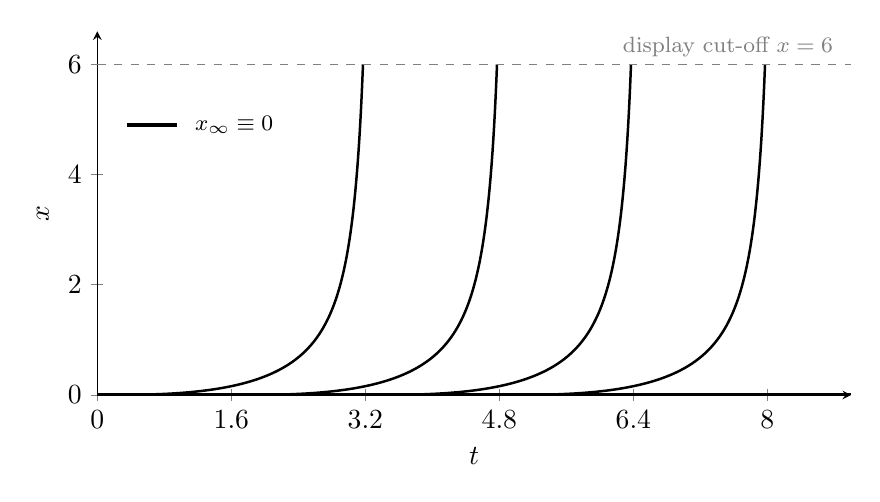
\begin{tikzpicture}
\begin{axis}[
  width=0.92\textwidth, height=6.2cm,
  xlabel={$t$}, ylabel={$x$},
  xmin=0, xmax=9, ymin=0, ymax=6.6,
  ytick={0,2,4,6},
  xtick={0,1.6,3.2,4.8,6.4,8},
  axis lines=left,
  every axis plot/.append style={line width=0.9pt},
  clip mode=individual,
]
\pgfplotsset{branch/.style={black, line width=0.9pt}}
\addplot[black, line width=1.3pt, domain=0:9] {0};
% generated by make_figure_data.py -- do not edit by hand
\addplot[branch] coordinates {(0.0,0.0) (0.09795276,3.48086e-5) (0.1628438,0.0001599383) (0.2192316,0.0003902593) (0.2707208,0.0007348835) (0.318848,0.001200661) (0.3644535,0.001793161) (0.4080615,0.00251711) (0.4500272,0.003376638) (0.4906056,0.004375423) (0.5299873,0.005516791) (0.5683198,0.006803783) (0.60572,0.008239204) (0.6422823,0.009825664) (0.6780844,0.0115656) (0.7131912,0.01346131) (0.7476573,0.01551495) (0.7815293,0.01772859) (0.8148474,0.02010416) (0.8476461,0.02264355) (0.8799558,0.02534851) (0.9118027,0.02822078) (0.9432102,0.03126198) (0.9741988,0.03447369) (1.004787,0.03785744) (1.03499,0.0414147) (1.064824,0.04514689) (1.0943,0.0490554) (1.12343,0.05314155) (1.152226,0.05740664) (1.180695,0.06185193) (1.208846,0.06647866) (1.236687,0.07128801) (1.264225,0.07628114) (1.291464,0.0814592) (1.318412,0.08682329) (1.345072,0.09237448) (1.371449,0.09811385) (1.397547,0.1040424) (1.423369,0.1101612) (1.448918,0.1164712) (1.474198,0.1229733) (1.49921,0.1296686) (1.523958,0.136558) (1.548442,0.1436423) (1.572666,0.1509225) (1.59663,0.1583995) (1.620335,0.1660741) (1.643784,0.1739471) (1.666977,0.1820195) (1.689915,0.190292) (1.7126,0.1987655) (1.735032,0.2074407) (1.757211,0.2163184) (1.77914,0.2253994) (1.800818,0.2346845) (1.822246,0.2441744) (1.843425,0.2538699) (1.864355,0.2637716) (1.885038,0.2738804) (1.905473,0.2841969) (1.925662,0.2947217) (1.945605,0.3054557) (1.965302,0.3163995) (1.984755,0.3275537) (2.003964,0.338919) (2.02293,0.3504961) (2.041655,0.3622856) (2.060137,0.3742882) (2.07838,0.3865045) (2.096384,0.3989351) (2.114149,0.4115806) (2.131677,0.4244417) (2.148969,0.4375189) (2.166026,0.4508129) (2.182849,0.4643242) (2.199441,0.4780534) (2.215801,0.4920011) (2.231933,0.506168) (2.247836,0.5205544) (2.263513,0.535161) (2.278965,0.5499884) (2.294194,0.5650371) (2.309202,0.5803077) (2.32399,0.5958006) (2.338561,0.6115165) (2.352915,0.6274558) (2.367056,0.643619) (2.380984,0.6600068) (2.394703,0.6766195) (2.408213,0.6934578) (2.421518,0.7105221) (2.434619,0.7278129) (2.447518,0.7453307) (2.460217,0.763076) (2.472719,0.7810493) (2.485027,0.7992511) (2.497141,0.8176818) (2.509065,0.836342) (2.520801,0.855232) (2.532351,0.8743524) (2.543717,0.8937037) (2.554902,0.9132862) (2.565908,0.9331005) (2.576737,0.953147) (2.587392,0.9734261) (2.597876,0.9939383) (2.60819,1.014684) (2.618337,1.035664) (2.628319,1.056878) (2.638139,1.078327) (2.647799,1.100011) (2.657301,1.121931) (2.666648,1.144087) (2.675842,1.16648) (2.684885,1.189109) (2.69378,1.211976) (2.702529,1.235081) (2.711134,1.258424) (2.719598,1.282005) (2.727922,1.305826) (2.73611,1.329886) (2.744162,1.354185) (2.752082,1.378725) (2.759872,1.403506) (2.767533,1.428527) (2.775068,1.45379) (2.782479,1.479295) (2.789768,1.505041) (2.796938,1.531031) (2.803989,1.557263) (2.810924,1.583738) (2.817746,1.610457) (2.824455,1.63742) (2.831055,1.664628) (2.837546,1.69208) (2.843932,1.719777) (2.850212,1.74772) (2.856391,1.775908) (2.862468,1.804343) (2.868447,1.833024) (2.874328,1.861952) (2.880114,1.891128) (2.885806,1.920551) (2.891406,1.950222) (2.896915,1.980141) (2.902335,2.010309) (2.907668,2.040726) (2.912916,2.071392) (2.918079,2.102308) (2.923159,2.133474) (2.928159,2.16489) (2.933078,2.196557) (2.937919,2.228474) (2.942684,2.260644) (2.947373,2.293064) (2.951987,2.325737) (2.956529,2.358662) (2.960999,2.39184) (2.965399,2.425271) (2.969731,2.458954) (2.973994,2.492892) (2.978191,2.527083) (2.982323,2.561529) (2.98639,2.596229) (2.990395,2.631184) (2.994338,2.666394) (2.99822,2.701859) (3.002042,2.737581) (3.005806,2.773558) (3.009513,2.809792) (3.013163,2.846282) (3.016757,2.88303) (3.020298,2.920034) (3.023784,2.957296) (3.027218,2.994817) (3.030601,3.032595) (3.033933,3.070632) (3.037215,3.108927) (3.040448,3.147482) (3.043634,3.186295) (3.046772,3.225369) (3.049864,3.264702) (3.05291,3.304296) (3.055911,3.34415) (3.058869,3.384265) (3.061784,3.424641) (3.064656,3.465278) (3.067487,3.506177) (3.070276,3.547337) (3.073026,3.58876) (3.075736,3.630446) (3.078407,3.672394) (3.08104,3.714605) (3.083636,3.757079) (3.086195,3.799817) (3.088717,3.842819) (3.091204,3.886084) (3.093656,3.929614) (3.096074,3.973409) (3.098458,4.017469) (3.100809,4.061794) (3.103127,4.106384) (3.105414,4.15124) (3.107668,4.196361) (3.109892,4.241749) (3.112085,4.287404) (3.114249,4.333325) (3.116383,4.379513) (3.118487,4.425969) (3.120564,4.472692) (3.122612,4.519682) (3.124633,4.566941) (3.126627,4.614468) (3.128595,4.662264) (3.130536,4.710328) (3.132451,4.758661) (3.134341,4.807264) (3.136206,4.856136) (3.138047,4.905277) (3.139863,4.954689) (3.141656,5.004371) (3.143426,5.054324) (3.145172,5.104547) (3.146896,5.155041) (3.148598,5.205807) (3.150278,5.256844) (3.151937,5.308153) (3.153574,5.359733) (3.155191,5.411586) (3.156787,5.463711) (3.158362,5.516109) (3.159918,5.56878) (3.161455,5.621724) (3.162972,5.674942) (3.16447,5.728433) (3.16595,5.782198) (3.167412,5.836236) (3.168855,5.89055) (3.17028,5.945137) (3.171689,6.0)};
\addplot[branch] coordinates {(0.0,0.0) (1.6,0.0) (1.697953,3.48086e-5) (1.762844,0.0001599383) (1.819232,0.0003902593) (1.870721,0.0007348835) (1.918848,0.001200661) (1.964453,0.001793161) (2.008061,0.00251711) (2.050027,0.003376638) (2.090606,0.004375423) (2.129987,0.005516791) (2.16832,0.006803783) (2.20572,0.008239204) (2.242282,0.009825664) (2.278084,0.0115656) (2.313191,0.01346131) (2.347657,0.01551495) (2.381529,0.01772859) (2.414847,0.02010416) (2.447646,0.02264355) (2.479956,0.02534851) (2.511803,0.02822078) (2.54321,0.03126198) (2.574199,0.03447369) (2.604787,0.03785744) (2.63499,0.0414147) (2.664824,0.04514689) (2.6943,0.0490554) (2.72343,0.05314155) (2.752226,0.05740664) (2.780695,0.06185193) (2.808846,0.06647866) (2.836687,0.07128801) (2.864225,0.07628114) (2.891464,0.0814592) (2.918412,0.08682329) (2.945072,0.09237448) (2.971449,0.09811385) (2.997547,0.1040424) (3.023369,0.1101612) (3.048918,0.1164712) (3.074198,0.1229733) (3.09921,0.1296686) (3.123958,0.136558) (3.148442,0.1436423) (3.172666,0.1509225) (3.19663,0.1583995) (3.220335,0.1660741) (3.243784,0.1739471) (3.266977,0.1820195) (3.289915,0.190292) (3.3126,0.1987655) (3.335032,0.2074407) (3.357211,0.2163184) (3.37914,0.2253994) (3.400818,0.2346845) (3.422246,0.2441744) (3.443425,0.2538699) (3.464355,0.2637716) (3.485038,0.2738804) (3.505473,0.2841969) (3.525662,0.2947217) (3.545605,0.3054557) (3.565302,0.3163995) (3.584755,0.3275537) (3.603964,0.338919) (3.62293,0.3504961) (3.641655,0.3622856) (3.660137,0.3742882) (3.67838,0.3865045) (3.696384,0.3989351) (3.714149,0.4115806) (3.731677,0.4244417) (3.748969,0.4375189) (3.766026,0.4508129) (3.782849,0.4643242) (3.799441,0.4780534) (3.815801,0.4920011) (3.831933,0.506168) (3.847836,0.5205544) (3.863513,0.535161) (3.878965,0.5499884) (3.894194,0.5650371) (3.909202,0.5803077) (3.92399,0.5958006) (3.938561,0.6115165) (3.952915,0.6274558) (3.967056,0.643619) (3.980984,0.6600068) (3.994703,0.6766195) (4.008213,0.6934578) (4.021518,0.7105221) (4.034619,0.7278129) (4.047518,0.7453307) (4.060217,0.763076) (4.072719,0.7810493) (4.085027,0.7992511) (4.097141,0.8176818) (4.109065,0.836342) (4.120801,0.855232) (4.132351,0.8743524) (4.143717,0.8937037) (4.154902,0.9132862) (4.165908,0.9331005) (4.176737,0.953147) (4.187392,0.9734261) (4.197876,0.9939383) (4.20819,1.014684) (4.218337,1.035664) (4.228319,1.056878) (4.238139,1.078327) (4.247799,1.100011) (4.257301,1.121931) (4.266648,1.144087) (4.275842,1.16648) (4.284885,1.189109) (4.29378,1.211976) (4.302529,1.235081) (4.311134,1.258424) (4.319598,1.282005) (4.327922,1.305826) (4.33611,1.329886) (4.344162,1.354185) (4.352082,1.378725) (4.359872,1.403506) (4.367533,1.428527) (4.375068,1.45379) (4.382479,1.479295) (4.389768,1.505041) (4.396938,1.531031) (4.403989,1.557263) (4.410924,1.583738) (4.417746,1.610457) (4.424455,1.63742) (4.431055,1.664628) (4.437546,1.69208) (4.443932,1.719777) (4.450212,1.74772) (4.456391,1.775908) (4.462468,1.804343) (4.468447,1.833024) (4.474328,1.861952) (4.480114,1.891128) (4.485806,1.920551) (4.491406,1.950222) (4.496915,1.980141) (4.502335,2.010309) (4.507668,2.040726) (4.512916,2.071392) (4.518079,2.102308) (4.523159,2.133474) (4.528159,2.16489) (4.533078,2.196557) (4.537919,2.228474) (4.542684,2.260644) (4.547373,2.293064) (4.551987,2.325737) (4.556529,2.358662) (4.560999,2.39184) (4.565399,2.425271) (4.569731,2.458954) (4.573994,2.492892) (4.578191,2.527083) (4.582323,2.561529) (4.58639,2.596229) (4.590395,2.631184) (4.594338,2.666394) (4.59822,2.701859) (4.602042,2.737581) (4.605806,2.773558) (4.609513,2.809792) (4.613163,2.846282) (4.616757,2.88303) (4.620298,2.920034) (4.623784,2.957296) (4.627218,2.994817) (4.630601,3.032595) (4.633933,3.070632) (4.637215,3.108927) (4.640448,3.147482) (4.643634,3.186295) (4.646772,3.225369) (4.649864,3.264702) (4.65291,3.304296) (4.655911,3.34415) (4.658869,3.384265) (4.661784,3.424641) (4.664656,3.465278) (4.667487,3.506177) (4.670276,3.547337) (4.673026,3.58876) (4.675736,3.630446) (4.678407,3.672394) (4.68104,3.714605) (4.683636,3.757079) (4.686195,3.799817) (4.688717,3.842819) (4.691204,3.886084) (4.693656,3.929614) (4.696074,3.973409) (4.698458,4.017469) (4.700809,4.061794) (4.703127,4.106384) (4.705414,4.15124) (4.707668,4.196361) (4.709892,4.241749) (4.712085,4.287404) (4.714249,4.333325) (4.716383,4.379513) (4.718487,4.425969) (4.720564,4.472692) (4.722612,4.519682) (4.724633,4.566941) (4.726627,4.614468) (4.728595,4.662264) (4.730536,4.710328) (4.732451,4.758661) (4.734341,4.807264) (4.736206,4.856136) (4.738047,4.905277) (4.739863,4.954689) (4.741656,5.004371) (4.743426,5.054324) (4.745172,5.104547) (4.746896,5.155041) (4.748598,5.205807) (4.750278,5.256844) (4.751937,5.308153) (4.753574,5.359733) (4.755191,5.411586) (4.756787,5.463711) (4.758362,5.516109) (4.759918,5.56878) (4.761455,5.621724) (4.762972,5.674942) (4.76447,5.728433) (4.76595,5.782198) (4.767412,5.836236) (4.768855,5.89055) (4.77028,5.945137) (4.771689,6.0)};
\addplot[branch] coordinates {(0.0,0.0) (3.2,0.0) (3.297953,3.48086e-5) (3.362844,0.0001599383) (3.419232,0.0003902593) (3.470721,0.0007348835) (3.518848,0.001200661) (3.564453,0.001793161) (3.608061,0.00251711) (3.650027,0.003376638) (3.690606,0.004375423) (3.729987,0.005516791) (3.76832,0.006803783) (3.80572,0.008239204) (3.842282,0.009825664) (3.878084,0.0115656) (3.913191,0.01346131) (3.947657,0.01551495) (3.981529,0.01772859) (4.014847,0.02010416) (4.047646,0.02264355) (4.079956,0.02534851) (4.111803,0.02822078) (4.14321,0.03126198) (4.174199,0.03447369) (4.204787,0.03785744) (4.23499,0.0414147) (4.264824,0.04514689) (4.2943,0.0490554) (4.32343,0.05314155) (4.352226,0.05740664) (4.380695,0.06185193) (4.408846,0.06647866) (4.436687,0.07128801) (4.464225,0.07628114) (4.491464,0.0814592) (4.518412,0.08682329) (4.545072,0.09237448) (4.571449,0.09811385) (4.597547,0.1040424) (4.623369,0.1101612) (4.648918,0.1164712) (4.674198,0.1229733) (4.69921,0.1296686) (4.723958,0.136558) (4.748442,0.1436423) (4.772666,0.1509225) (4.79663,0.1583995) (4.820335,0.1660741) (4.843784,0.1739471) (4.866977,0.1820195) (4.889915,0.190292) (4.9126,0.1987655) (4.935032,0.2074407) (4.957211,0.2163184) (4.97914,0.2253994) (5.000818,0.2346845) (5.022246,0.2441744) (5.043425,0.2538699) (5.064355,0.2637716) (5.085038,0.2738804) (5.105473,0.2841969) (5.125662,0.2947217) (5.145605,0.3054557) (5.165302,0.3163995) (5.184755,0.3275537) (5.203964,0.338919) (5.22293,0.3504961) (5.241655,0.3622856) (5.260137,0.3742882) (5.27838,0.3865045) (5.296384,0.3989351) (5.314149,0.4115806) (5.331677,0.4244417) (5.348969,0.4375189) (5.366026,0.4508129) (5.382849,0.4643242) (5.399441,0.4780534) (5.415801,0.4920011) (5.431933,0.506168) (5.447836,0.5205544) (5.463513,0.535161) (5.478965,0.5499884) (5.494194,0.5650371) (5.509202,0.5803077) (5.52399,0.5958006) (5.538561,0.6115165) (5.552915,0.6274558) (5.567056,0.643619) (5.580984,0.6600068) (5.594703,0.6766195) (5.608213,0.6934578) (5.621518,0.7105221) (5.634619,0.7278129) (5.647518,0.7453307) (5.660217,0.763076) (5.672719,0.7810493) (5.685027,0.7992511) (5.697141,0.8176818) (5.709065,0.836342) (5.720801,0.855232) (5.732351,0.8743524) (5.743717,0.8937037) (5.754902,0.9132862) (5.765908,0.9331005) (5.776737,0.953147) (5.787392,0.9734261) (5.797876,0.9939383) (5.80819,1.014684) (5.818337,1.035664) (5.828319,1.056878) (5.838139,1.078327) (5.847799,1.100011) (5.857301,1.121931) (5.866648,1.144087) (5.875842,1.16648) (5.884885,1.189109) (5.89378,1.211976) (5.902529,1.235081) (5.911134,1.258424) (5.919598,1.282005) (5.927922,1.305826) (5.93611,1.329886) (5.944162,1.354185) (5.952082,1.378725) (5.959872,1.403506) (5.967533,1.428527) (5.975068,1.45379) (5.982479,1.479295) (5.989768,1.505041) (5.996938,1.531031) (6.003989,1.557263) (6.010924,1.583738) (6.017746,1.610457) (6.024455,1.63742) (6.031055,1.664628) (6.037546,1.69208) (6.043932,1.719777) (6.050212,1.74772) (6.056391,1.775908) (6.062468,1.804343) (6.068447,1.833024) (6.074328,1.861952) (6.080114,1.891128) (6.085806,1.920551) (6.091406,1.950222) (6.096915,1.980141) (6.102335,2.010309) (6.107668,2.040726) (6.112916,2.071392) (6.118079,2.102308) (6.123159,2.133474) (6.128159,2.16489) (6.133078,2.196557) (6.137919,2.228474) (6.142684,2.260644) (6.147373,2.293064) (6.151987,2.325737) (6.156529,2.358662) (6.160999,2.39184) (6.165399,2.425271) (6.169731,2.458954) (6.173994,2.492892) (6.178191,2.527083) (6.182323,2.561529) (6.18639,2.596229) (6.190395,2.631184) (6.194338,2.666394) (6.19822,2.701859) (6.202042,2.737581) (6.205806,2.773558) (6.209513,2.809792) (6.213163,2.846282) (6.216757,2.88303) (6.220298,2.920034) (6.223784,2.957296) (6.227218,2.994817) (6.230601,3.032595) (6.233933,3.070632) (6.237215,3.108927) (6.240448,3.147482) (6.243634,3.186295) (6.246772,3.225369) (6.249864,3.264702) (6.25291,3.304296) (6.255911,3.34415) (6.258869,3.384265) (6.261784,3.424641) (6.264656,3.465278) (6.267487,3.506177) (6.270276,3.547337) (6.273026,3.58876) (6.275736,3.630446) (6.278407,3.672394) (6.28104,3.714605) (6.283636,3.757079) (6.286195,3.799817) (6.288717,3.842819) (6.291204,3.886084) (6.293656,3.929614) (6.296074,3.973409) (6.298458,4.017469) (6.300809,4.061794) (6.303127,4.106384) (6.305414,4.15124) (6.307668,4.196361) (6.309892,4.241749) (6.312085,4.287404) (6.314249,4.333325) (6.316383,4.379513) (6.318487,4.425969) (6.320564,4.472692) (6.322612,4.519682) (6.324633,4.566941) (6.326627,4.614468) (6.328595,4.662264) (6.330536,4.710328) (6.332451,4.758661) (6.334341,4.807264) (6.336206,4.856136) (6.338047,4.905277) (6.339863,4.954689) (6.341656,5.004371) (6.343426,5.054324) (6.345172,5.104547) (6.346896,5.155041) (6.348598,5.205807) (6.350278,5.256844) (6.351937,5.308153) (6.353574,5.359733) (6.355191,5.411586) (6.356787,5.463711) (6.358362,5.516109) (6.359918,5.56878) (6.361455,5.621724) (6.362972,5.674942) (6.36447,5.728433) (6.36595,5.782198) (6.367412,5.836236) (6.368855,5.89055) (6.37028,5.945137) (6.371689,6.0)};
\addplot[branch] coordinates {(0.0,0.0) (4.8,0.0) (4.897953,3.48086e-5) (4.962844,0.0001599383) (5.019232,0.0003902593) (5.070721,0.0007348835) (5.118848,0.001200661) (5.164453,0.001793161) (5.208061,0.00251711) (5.250027,0.003376638) (5.290606,0.004375423) (5.329987,0.005516791) (5.36832,0.006803783) (5.40572,0.008239204) (5.442282,0.009825664) (5.478084,0.0115656) (5.513191,0.01346131) (5.547657,0.01551495) (5.581529,0.01772859) (5.614847,0.02010416) (5.647646,0.02264355) (5.679956,0.02534851) (5.711803,0.02822078) (5.74321,0.03126198) (5.774199,0.03447369) (5.804787,0.03785744) (5.83499,0.0414147) (5.864824,0.04514689) (5.8943,0.0490554) (5.92343,0.05314155) (5.952226,0.05740664) (5.980695,0.06185193) (6.008846,0.06647866) (6.036687,0.07128801) (6.064225,0.07628114) (6.091464,0.0814592) (6.118412,0.08682329) (6.145072,0.09237448) (6.171449,0.09811385) (6.197547,0.1040424) (6.223369,0.1101612) (6.248918,0.1164712) (6.274198,0.1229733) (6.29921,0.1296686) (6.323958,0.136558) (6.348442,0.1436423) (6.372666,0.1509225) (6.39663,0.1583995) (6.420335,0.1660741) (6.443784,0.1739471) (6.466977,0.1820195) (6.489915,0.190292) (6.5126,0.1987655) (6.535032,0.2074407) (6.557211,0.2163184) (6.57914,0.2253994) (6.600818,0.2346845) (6.622246,0.2441744) (6.643425,0.2538699) (6.664355,0.2637716) (6.685038,0.2738804) (6.705473,0.2841969) (6.725662,0.2947217) (6.745605,0.3054557) (6.765302,0.3163995) (6.784755,0.3275537) (6.803964,0.338919) (6.82293,0.3504961) (6.841655,0.3622856) (6.860137,0.3742882) (6.87838,0.3865045) (6.896384,0.3989351) (6.914149,0.4115806) (6.931677,0.4244417) (6.948969,0.4375189) (6.966026,0.4508129) (6.982849,0.4643242) (6.999441,0.4780534) (7.015801,0.4920011) (7.031933,0.506168) (7.047836,0.5205544) (7.063513,0.535161) (7.078965,0.5499884) (7.094194,0.5650371) (7.109202,0.5803077) (7.12399,0.5958006) (7.138561,0.6115165) (7.152915,0.6274558) (7.167056,0.643619) (7.180984,0.6600068) (7.194703,0.6766195) (7.208213,0.6934578) (7.221518,0.7105221) (7.234619,0.7278129) (7.247518,0.7453307) (7.260217,0.763076) (7.272719,0.7810493) (7.285027,0.7992511) (7.297141,0.8176818) (7.309065,0.836342) (7.320801,0.855232) (7.332351,0.8743524) (7.343717,0.8937037) (7.354902,0.9132862) (7.365908,0.9331005) (7.376737,0.953147) (7.387392,0.9734261) (7.397876,0.9939383) (7.40819,1.014684) (7.418337,1.035664) (7.428319,1.056878) (7.438139,1.078327) (7.447799,1.100011) (7.457301,1.121931) (7.466648,1.144087) (7.475842,1.16648) (7.484885,1.189109) (7.49378,1.211976) (7.502529,1.235081) (7.511134,1.258424) (7.519598,1.282005) (7.527922,1.305826) (7.53611,1.329886) (7.544162,1.354185) (7.552082,1.378725) (7.559872,1.403506) (7.567533,1.428527) (7.575068,1.45379) (7.582479,1.479295) (7.589768,1.505041) (7.596938,1.531031) (7.603989,1.557263) (7.610924,1.583738) (7.617746,1.610457) (7.624455,1.63742) (7.631055,1.664628) (7.637546,1.69208) (7.643932,1.719777) (7.650212,1.74772) (7.656391,1.775908) (7.662468,1.804343) (7.668447,1.833024) (7.674328,1.861952) (7.680114,1.891128) (7.685806,1.920551) (7.691406,1.950222) (7.696915,1.980141) (7.702335,2.010309) (7.707668,2.040726) (7.712916,2.071392) (7.718079,2.102308) (7.723159,2.133474) (7.728159,2.16489) (7.733078,2.196557) (7.737919,2.228474) (7.742684,2.260644) (7.747373,2.293064) (7.751987,2.325737) (7.756529,2.358662) (7.760999,2.39184) (7.765399,2.425271) (7.769731,2.458954) (7.773994,2.492892) (7.778191,2.527083) (7.782323,2.561529) (7.78639,2.596229) (7.790395,2.631184) (7.794338,2.666394) (7.79822,2.701859) (7.802042,2.737581) (7.805806,2.773558) (7.809513,2.809792) (7.813163,2.846282) (7.816757,2.88303) (7.820298,2.920034) (7.823784,2.957296) (7.827218,2.994817) (7.830601,3.032595) (7.833933,3.070632) (7.837215,3.108927) (7.840448,3.147482) (7.843634,3.186295) (7.846772,3.225369) (7.849864,3.264702) (7.85291,3.304296) (7.855911,3.34415) (7.858869,3.384265) (7.861784,3.424641) (7.864656,3.465278) (7.867487,3.506177) (7.870276,3.547337) (7.873026,3.58876) (7.875736,3.630446) (7.878407,3.672394) (7.88104,3.714605) (7.883636,3.757079) (7.886195,3.799817) (7.888717,3.842819) (7.891204,3.886084) (7.893656,3.929614) (7.896074,3.973409) (7.898458,4.017469) (7.900809,4.061794) (7.903127,4.106384) (7.905414,4.15124) (7.907668,4.196361) (7.909892,4.241749) (7.912085,4.287404) (7.914249,4.333325) (7.916383,4.379513) (7.918487,4.425969) (7.920564,4.472692) (7.922612,4.519682) (7.924633,4.566941) (7.926627,4.614468) (7.928595,4.662264) (7.930536,4.710328) (7.932451,4.758661) (7.934341,4.807264) (7.936206,4.856136) (7.938047,4.905277) (7.939863,4.954689) (7.941656,5.004371) (7.943426,5.054324) (7.945172,5.104547) (7.946896,5.155041) (7.948598,5.205807) (7.950278,5.256844) (7.951937,5.308153) (7.953574,5.359733) (7.955191,5.411586) (7.956787,5.463711) (7.958362,5.516109) (7.959918,5.56878) (7.961455,5.621724) (7.962972,5.674942) (7.96447,5.728433) (7.96595,5.782198) (7.967412,5.836236) (7.968855,5.89055) (7.97028,5.945137) (7.971689,6.0)};

\draw[dashed, gray] (axis cs:0,6) -- (axis cs:9,6);
\node[anchor=east, font=\footnotesize, gray] at (axis cs:8.9,6.32)
      {display cut-off $x=6$};
\draw[black, line width=1.3pt] (axis cs:0.35,4.9) -- (axis cs:0.95,4.9);
\node[anchor=west, font=\footnotesize] at (axis cs:1.05,4.9) {$x_{\infty}\equiv 0$};
\end{axis}
\end{tikzpicture}
\caption{Four members of the family, departing at $T=0,\,1.6,\,3.2,\,4.8$. Each
curve is $\varphi$, traced \emph{for the drawing only} by sampling $x$ and
plotting $\big(T+F(x),\,x\big)$, so that $F$ is evaluated and never inverted;
the blow-up time is the analytic $T_{*}$ of
Proposition~\ref{prop:Tstar}, and nothing here is offered as evidence for it.
The curves are drawn only up to $x=6$; that ceiling is graphical, and each
branch in fact runs to $+\infty$ as $t$ approaches $T+T_{*}$. Along the axis is
$x_{\infty}$, the one solution still defined at every later time.}
\label{fig:branches}
\end{figure}

%------------------------------------------------------------------
\section{Globally defined versus forward-maximal}\label{sec:counts}

Two classes of forward solution, kept apart.

\begin{definition}\label{def:classes}
$\Hglob(0)$ is the set of solutions of \eqref{eq:ivp} defined at \emph{every}
$t\ge0$, that is, those with $I=[0,\infty)$.

$\Hmax(0)$ is the set of solutions of \eqref{eq:ivp} on intervals
$I\subseteq[0,\infty)$ admitting no extension to a solution on a strictly larger
$J\subseteq[0,\infty)$. We call these \emph{forward-maximal};
Section~\ref{sec:senses} explains why the prefix is not optional.
\end{definition}

Plainly $\Hglob(0)\subseteq\Hmax(0)$: a solution on $[0,\infty)$ has nowhere
further to go inside $[0,\infty)$. The main statement is that the two classes
are nevertheless as far apart as they could be.

\begin{theorem}\label{thm:counts}
Assume \textup{(H1)--(H3)}. Then, with $\Hmax(0)$ the \emph{forward}-maximal
solutions of Definition~\ref{def:classes} --- not the two-sided maximal
solutions of Section~\ref{sec:senses} ---
\[
  \Hglob(0)=\{x_{\infty}\},
  \qquad
  \Hmax(0)=\{x_{T}: T\in[0,\infty)\}\cup\{x_{\infty}\},
\]
so that $|\Hglob(0)|=1$ while $|\Hmax(0)|=\cont$.
\end{theorem}

\begin{proof}
We argue in eight steps.

\smallskip
\emph{Step 1 (monotonicity).} Since $f\ge0$ everywhere, every solution has
$\dot x\ge0$ and so is non-decreasing; as $x(0)=0$, every solution is
non-negative.

\smallskip
\emph{Step 2 (the zero set).} Let $x$ be a solution on $I$ and put
$Z=\{t\in I: x(t)=0\}$. Then $Z$ is closed in $I$ by continuity, and is an
interval: if $t_{1}<t<t_{2}$ with $t_{1},t_{2}\in Z$ then
$0=x(t_{1})\le x(t)\le x(t_{2})=0$ by Step 1. Also $0\in Z$. Set
$T=\sup Z\in[0,\infty]$.

\smallskip
\emph{Step 3 (each $x_{T}$ is forward-maximal).} By Lemma~\ref{lem:phi},
$x_{T}(t)\to+\infty$ as $t\to(T+T_{*})^{-}$. Any $J\subseteq[0,\infty)$ strictly
containing $I=[0,T+T_{*})$ and admitting a solution extending $x_{T}$ would have
to contain the point $T+T_{*}$, at which the extension would have to be finite
and continuous --- impossible. So $x_{T}\in\Hmax(0)$. Likewise
$x_{\infty}\in\Hglob(0)\subseteq\Hmax(0)$.

\smallskip
\emph{Step 4 (no forward-maximal solution has a compact domain).} Suppose
$x\in\Hmax(0)$ has $I=[0,b]$ with $b<\infty$. Then $x(b)$ is finite and $f$ is
continuous, so Peano's existence theorem supplies a solution $y$ of
$\dot y=f(y)$ on some $[b,b+\delta]$ with $y(b)=x(b)$. Concatenating $x$ and $y$
gives a solution on $[0,b+\delta]$ properly extending $x$, contradicting
maximality. Hence every $I$ arising in $\Hmax(0)$ is right-open or is
$[0,\infty)$.

\smallskip
\emph{Step 5 (the case $T=\infty$).} If $T=\infty$ then $Z$ is unbounded, and
being an interval containing $0$ it equals $I$; so $x\equiv0$ on $I$. If
$I\ne[0,\infty)$ then extending by $0$ gives a solution on a strictly larger
subinterval of $[0,\infty)$, contradicting maximality. So $I=[0,\infty)$ and
$x=x_{\infty}$.

\smallskip
\emph{Step 6 (the case $T<\infty$).} First, $T\in I$. Otherwise $I$ is an
interval containing $[0,T)$ but not $T$, hence $I\subseteq[0,T)$ and $x\equiv0$
on $I$, so $x(t)\to0$ as $t\uparrow T$. Setting $x(T)=0$ extends $x$
continuously to $[0,T]$, and the extension solves \eqref{eq:ivp} at $T$ because
$f(0)=0$; it is then extended further by the zero solution. This contradicts
maximality. (Step 4 handles the general version of the same situation: at a
compact right endpoint at which the solution is finite, Peano's existence
theorem gives a local solution from that value, which concatenates to a proper
extension. Here the value is the equilibrium, so the extension is the zero
solution and no appeal to Peano is needed.)

For $t\in I$ with $t>T$ we have $x(t)\ne0$ by the definition of $T$ as
$\sup Z$, and $x(t)\ge x(T)=0$ by Step 1; hence $x(t)>0$. On $I\cap(T,\infty)$
therefore $\dot x=f(x)>0$, so $x$ is strictly increasing there and
$\dot x/f(x)=1$. Integrating from $s$ to $t$ with $T<s<t$ and substituting
$u=x(\sigma)$ --- legitimate since $x$ is a $C^{1}$ strictly increasing
bijection from $[s,t]$ onto $[x(s),x(t)]$ --- gives
\[
  t-s=\int_{s}^{t}\frac{\dot x(\sigma)}{f(x(\sigma))}\,d\sigma
     =\int_{x(s)}^{x(t)}\frac{du}{f(u)}
     =F(x(t))-F(x(s)).
\]
Letting $s\downarrow T$ and using $x(s)\to x(T)=0$ together with $F(0^{+})=0$
yields $F(x(t))=t-T$, that is $x(t)=\varphi(t-T)$. Since $F$ takes values in
$(0,T_{*})$ this forces $t-T<T_{*}$, so $I\subseteq[0,T+T_{*})$. By Step 4 the
domain is not compact, and by maximality together with Step 3 it cannot be a
proper subinterval of $[0,T+T_{*})$; hence $I=[0,T+T_{*})$ and $x=x_{T}$.

\smallskip
\emph{Step 7 (the cardinality of $\Hmax(0)$).} Steps 3, 5 and 6 together give
the stated description of $\Hmax(0)$. For the lower bound, $T\mapsto x_{T}$ is
injective: if $T_{1}<T_{2}$ then on the interval $(T_{1},T_{2}]$, of positive
length, $x_{T_{1}}=\varphi(\,\cdot-T_{1})>0$ while $x_{T_{2}}=0$, so the two
functions differ. Moreover $x_{\infty}\ne x_{T}$ for every $T<\infty$, since
$x_{\infty}\equiv0$ while $x_{T}>0$ on $(T,T+T_{*})$; so the listed solutions
are pairwise distinct and $|\Hmax(0)|\ge|[0,\infty)|=\cont$.

For the upper bound, every solution is a continuous real-valued function on a
subinterval of $[0,\infty)$. There are $\cont$ such subintervals, and a
continuous function on an interval is determined by its values on a countable
dense subset, so each interval carries at most $\cont^{\aleph_{0}}=\cont$ of
them. Hence $|\Hmax(0)|\le\cont\cdot\cont=\cont$. Combining the bounds,
$|\Hmax(0)|=\cont$.

\smallskip
\emph{Step 8 (the globally defined solutions).} Let $x\in\Hglob(0)$, so
$I=[0,\infty)$. A solution on $[0,\infty)$ admits no extension inside
$[0,\infty)$, so $\Hglob(0)\subseteq\Hmax(0)$ and $x$ is on the list above. It
is not any $x_{T}$ with $T<\infty$: by Lemma~\ref{lem:phi} such a branch
satisfies $x_{T}(t)\to+\infty$ as $t\uparrow T+T_{*}$, so it is defined only on
the bounded interval $[0,T+T_{*})$ and in particular not at $t=T+T_{*}$. Every
non-zero branch therefore reaches $+\infty$ after the finite additional time
$T_{*}$ and fails to be global. The only remaining possibility is
$x=x_{\infty}$, which is indeed defined on all of $[0,\infty)$. Hence
$\Hglob(0)=\{x_{\infty}\}$ and $|\Hglob(0)|=1$.
\end{proof}

\begin{remark}[The counts do not depend on the solution concept]\label{rem:AC}
Definition~\ref{def:solution} asks for a differentiable solution; Binding
\cite{Binding} works instead with absolutely continuous $x$ satisfying
$\dot x=f(x)$ almost everywhere. The two give the same sets here. If $x$ is
absolutely continuous with $\dot x=f(x)$ a.e., then
$x(t)=x(0)+\int_{0}^{t}f(x(s))\,ds$, and $f\circ x$ is continuous, so $x$ is
$C^{1}$ and solves \eqref{eq:ivp} in the classical sense. So
Theorem~\ref{thm:counts} is not an artefact of the regularity demanded of
solutions.
\end{remark}

\begin{remark}[Each hypothesis moves one count]\label{rem:sensitivity}
Without (H2) no branch could leave the origin, and both counts would be $1$;
without (H3) every $x_{T}$ would be defined on all of $[0,\infty)$, and both
counts would be $\cont$. Only the conjunction separates them. The margin is also
the largest available, and both ends of it are fixed. At the upper end, by
Step 7 no solution set of \eqref{eq:ivp} can exceed $\cont$. At the lower end,
(H1) gives $f(0)=0$, so $x_{\infty}\equiv0$ on $[0,\infty)$ satisfies
Definition~\ref{def:solution} and lies in $\Hglob(0)$; hence
$|\Hglob(0)|\ge1$ whenever (H1) holds. The pair $(1,\cont)$ of
Theorem~\ref{thm:counts} therefore realises the smallest global count together
with the largest forward-maximal one, and no instance of \eqref{eq:ivp}
satisfying (H1) can separate the two counts further.
\end{remark}

The remark can be stated exactly, and stating it exactly locates \emph{where}
each of the two verdicts is determined. The next proposition does no more than
read that off the three cases; its ingredients are the classical dichotomies
attributed in Section~\ref{sec:classical}, and we claim no priority for it.

\begin{proposition}[Where each verdict is determined]\label{prop:locality}
Assume \textup{(H1)}, but not necessarily \textup{(H2)} or \textup{(H3)}. Then
\[
  |\Hmax(0)|=1 \iff \neg\textup{(H2)},
  \qquad
  |\Hglob(0)|=1 \iff \neg\textup{(H2)}\ \vee\ \textup{(H3)} .
\]
The condition on the left is determined by the restriction of $f$ to any
neighbourhood of the origin. The condition on the right is not determined by the
restriction of $f$ to any bounded set.
\end{proposition}

\begin{proof}
Three cases exhaust the possibilities.

\smallskip
\emph{Case $\neg$\textup{(H2)}.} We claim $x\equiv0$ is the only solution. This
is the departure criterion recorded in Section~\ref{sec:classical}; the direct
argument is short enough to give, and keeps the proposition self-contained.
Suppose some solution $x$ on $I$ had $x(t_{0})>0$ for some $t_{0}\in I$. Steps 1
and 2 of Theorem~\ref{thm:counts} use only (H1), so $x$ is non-decreasing and
non-negative and $Z=\{t\in I:x(t)=0\}$ is an interval containing $0$. Since
$t_{0}\notin Z$, and $Z$ is an interval containing $0$, we get
$Z\subseteq[0,t_{0})$; hence $T:=\sup Z\le t_{0}<\infty$ and
$[0,T)\subseteq Z$. As $[0,t_{0}]\subseteq I$ we have $T\in I$, and $x(T)=0$ by
continuity; moreover $T<t_{0}$, since $x(T)=0<x(t_{0})$. And $x(s)>0$ for every
$s\in(T,t_{0}]$, since such an $s$ lies outside $Z$ while $x\ge0$. The computation in Step 6 of
Theorem~\ref{thm:counts} --- which uses only (H1) and the strict positivity of
$x$ on $I\cap(T,\infty)$, not (H2) or (H3) --- gives
\[
  t_{0}-s=\int_{x(s)}^{x(t_{0})}\frac{du}{f(u)}
  \qquad\text{for every } s\in(T,t_{0}) .
\]
Let $s\downarrow T$. The left-hand side tends to $t_{0}-T<\infty$. On the right,
$x(s)\to x(T)=0$ by continuity and $1/f>0$ on $(0,\infty)$, so the integral
increases to $\int_{0}^{x(t_{0})}du/f(u)$. That limit is $+\infty$. Indeed, put
$c=\min\big(1,x(t_{0})\big)>0$; all three terms in
$\int_{0}^{1}du/f=\int_{0}^{c}du/f+\int_{c}^{1}du/f$ are non-negative, the left
side is $+\infty$ by $\neg$(H2), and $\int_{c}^{1}du/f$ is finite because $1/f$
is continuous on the compact interval $[c,1]\subset(0,\infty)$; so
$\int_{0}^{c}du/f=+\infty$, and $\int_{0}^{x(t_{0})}du/f$ dominates it. This
contradicts $t_{0}-T<\infty$. Hence no solution takes a positive value, and with
Step 1 every solution is identically $0$ on its domain. The extension argument
inside Step 5 --- which also uses only (H1), and does not depend on that step's
case hypothesis --- then forces $I=[0,\infty)$ for a forward-maximal solution:
a solution identically $0$ on a proper subinterval of $[0,\infty)$ is properly
extended by the zero solution. So
$\Hmax(0)=\Hglob(0)=\{x_{\infty}\}$ and both counts are $1$.

\smallskip
\emph{Case \textup{(H2)} and \textup{(H3)}.} Theorem~\ref{thm:counts} gives
$|\Hmax(0)|=\cont$ and $|\Hglob(0)|=1$.

\smallskip
\emph{Case \textup{(H2)} and $\neg$\textup{(H3)}.} Then $F$ is a bijection from
$(0,\infty)$ onto $(0,\infty)$, so $\varphi$ is defined on all of $[0,\infty)$
and every $x_{T}$ is global; the argument of Theorem~\ref{thm:counts} is
otherwise unchanged, and $\Hmax(0)=\Hglob(0)=\{x_{T}:T\in[0,\infty)\}\cup
\{x_{\infty}\}$, of cardinality $\cont$.

\smallskip
Reading the two counts off the three cases gives the two equivalences.

\smallskip
\emph{The locality claims.} First, (H2) is determined by the restriction of $f$ to
$(0,\delta)$ for every $\delta\in(0,1]$: by (H1) $f>0$ on the compact interval
$[\delta,1]\subset(0,\infty)$, so $1/f$ is continuous and hence integrable
there, and therefore $\int_{0}^{1}du/f$ and $\int_{0}^{\delta}du/f$ converge
together. For $\delta>1$ the claim is immediate, since then
$(0,\delta)\supseteq(0,1)$. Equivalently: if two functions satisfying (H1) agree
on some neighbourhood of the origin, then either both satisfy (H2) or neither
does.

Second, (H3) is not determined by the restriction of $f$ to any bounded set. Every
bounded set is contained in $[-M,M]$ for some $M>0$, so it suffices to produce,
for each $M>0$, two functions satisfying (H1) that agree on the whole of
$[-M,M]$ and disagree about (H3). One pair agreeing on $[-1,1]$ would settle
only the case $M=1$. Take $f(x)=|x|^{2/3}+x^{2}$ as in
Section~\ref{sec:example}, fix $M>0$, and put
\[
  f^{\flat}_{M}(x)=\begin{cases}
    f(x), & |x|\le M,\\[2pt]
    f(M)\,|x|/M, & |x|\ge M .
  \end{cases}
\]
\emph{Continuity.} Each branch is continuous where it is defined, and at
$|x|=M$ the second reads $f(M)M/M=f(M)$, so the branches agree there; hence
$f^{\flat}_{M}$ is continuous on $\R$.

\emph{\textup{(H1)}.} The hypothesis asks for continuity, the value $0$ at the
origin, and positivity off the origin, and for nothing else. Continuity is just
shown; $f^{\flat}_{M}(0)=f(0)=0$, since $0\le M$; for $0<|x|\le M$ we have
$f^{\flat}_{M}(x)=f(x)>0$; and for $|x|\ge M$ we have
$f^{\flat}_{M}(x)=f(M)|x|/M>0$, because $f(M)=M^{2/3}+M^{2}>0$ and $M>0$.

\emph{\textup{(H2)} is preserved.} $f^{\flat}_{M}$ agrees with $f$ on
$[-\min(M,1),\min(M,1)]$, a neighbourhood of the origin, so by the paragraph
above it satisfies (H2) exactly when $f$ does --- which $f$ does, by
Lemma~\ref{lem:properties}(iv).

\emph{\textup{(H3)} fails.} Put $N=\max(M,1)$. On $[N,\infty)$ we have
$f^{\flat}_{M}(x)=f(M)x/M$, so
$\int_{N}^{\infty}dx/f^{\flat}_{M}=(M/f(M))\int_{N}^{\infty}dx/x=\infty$, while
$\int_{1}^{N}dx/f^{\flat}_{M}$ is finite, its integrand being continuous on the
compact interval $[1,N]\subset(0,\infty)$. Hence
$\int_{1}^{\infty}dx/f^{\flat}_{M}=\infty$.

\emph{Agreement.} By construction $f^{\flat}_{M}=f$ on the whole of $[-M,M]$.

So $f$ satisfies (H2) and (H3), while $f^{\flat}_{M}$ satisfies (H2) and not
(H3), and the two agree on $[-M,M]$. By the equivalences just proved,
$|\Hglob(0)|=1$ for $f$ and $|\Hglob(0)|=\cont$ for $f^{\flat}_{M}$, whereas
$|\Hmax(0)|=\cont$ for both. Since $M>0$ was arbitrary and every bounded set
lies in some $[-M,M]$, no bounded set determines (H3).
\end{proof}

So the two counts are not determined in the same place. Whether one solution or
continuum-many cannot be extended forward is settled by the law near the state;
whether
one solution or continuum-many are defined at every later time is not, and no
amount of information about the law near the state settles it.

One remark, to forestall a misreading. Proposition~\ref{prop:locality} locates
each condition in the coordinate $x$, in which the initial state and both
solution classes are posed; it does not say that finite-time escape has no local
description at all. The reciprocal substitution recorded in
Section~\ref{sec:classical} carries $\dot x=f(x)$ into
$\dot\alpha=-\hat f(\alpha)$ with $\hat f(\alpha)=\alpha^{2}f(1/\alpha)$, and
Binding's Lemma 6.3 records that escape to infinity for $f$ corresponds to
non-uniqueness at the origin for $\hat f$. Read in $\alpha$ instead of in $x$,
(H3) is again a condition at the origin; the contrast drawn by the proposition
is between two conditions read in two different coordinates, not between one
that has a local reading and one that has none.

%------------------------------------------------------------------
\section{Three senses of ``maximal''}\label{sec:senses}

The word carries at least three meanings in the surrounding literature, and
conflating them produces false statements about this example. We separate them
once and then keep the prefix.

\begin{itemize}
  \item \textbf{Forward-maximal:} no extension within $[0,\infty)$. These are the
        $x_{T}$, on $[0,T+T_{*})$ --- the class counted in
        Theorem~\ref{thm:counts}.
  \item \textbf{Maximal (standard):} no extension to any larger interval of $\R$.
        \emph{No $x_{T}$ is maximal in this sense.} Setting $x(t)=0$ for $t<0$
        always extends it, since $f(0)=0$. Appendix~\ref{app:twosided}
        classifies the genuinely maximal solutions.
  \item \textbf{Maximal (extremal):} the \emph{largest} solution pointwise on
        the common interval of existence --- the qualification matters here,
        since the candidates have different domains. That solution is $x_{0}$,
        which departs immediately; the smallest in the same sense is
        $x_{\infty}$. Hartman \cite[ch.~III \S2]{Hartman} uses the word in this
        sense.
\end{itemize}

So $[0,T+T_{*})$ is a forward-maximal interval and not a maximal interval, and
$\Hmax(0)$ is not a set of maximal solutions.

%------------------------------------------------------------------
\section{What is classical, and where}\label{sec:classical}

The results above rest on classical theory, and we claim no priority for any of
them. The attributions below are specific rather than general, because a general
gesture at ``the classical theory'' would leave a reader unable to check them.

\textbf{Wallach \cite{Wallach}, 1948.} Characterised \emph{all} solutions of
$\dot x=f\circ x$, $x(0)=0$ for continuous $f$. Binding reports this at
\cite[p.~184]{Binding} --- ``Wallach characterized all solutions of (1.1)'' ---
and credits the monotonicity lemma and the structure theorem to two sections of
it, which he cites as Wallach's \S2 and \S7 respectively. \emph{We know this
paper only through Binding and have not read it; the two section numbers are
Binding's citations, reproduced here, and we have not checked them against
Wallach.}

\textbf{Binding \cite[\S3, pp.~186--188]{Binding}.} The machinery of
Theorem~\ref{thm:counts}. Lemma 3.2: every solution is monotonic, which Binding
credits to Wallach \cite{Wallach} for continuous $f$ --- our Step 1.
Theorem 3.3: the separation identity
$\lambda([s,t]\setminus\dot x^{-1}(0))=\int_{x(s)}^{x(t)}1/f$ in
measure-theoretic form, of which the computation in Step 6 is the elementary
case. Theorem 3.5: necessary conditions for local existence, reducing for
continuous $f$ with $x>0$, in his words, to ``$f>0$ and $1/f$ integrable, as
given by Wallach''.

\textbf{Binding \cite[\S\S5--6, pp.~190--193]{Binding}.} Theorem 5.3 is the
uniqueness criterion, in the Osgood \cite{Osgood} and Kamke line --- Binding
names both on the same page --- and see Hartman \cite[ch.~III \S6]{Hartman},
where Theorem 6.1 is Kamke's and Corollary 6.2 is Osgood's. Fjordholm
\cite{Fjordholm}, whose own subject is Filippov uniqueness for discontinuous
fields, restates the continuous case as ``it was shown by Binding that the
solution is unique if and only if $b$ satisfies the so-called Osgood condition
at all zeroes of $b$''. Binding's case (6.5) corresponds to (H2) and (H3)
together,
not to (H3) alone: the integral in that case runs from the equilibrium, so its
convergence near the origin is (H2) and its convergence at infinity is (H3).
With (H2) standing, as it does throughout this note, it is (H3) that does the
work. Of that case Binding writes, ``we have the phenomenon of escape to
infinity for at least one solution''; Binding's case (6.2), where the integral
diverges, is the complementary one in which the branch survives on the whole
half-line. Lemma 6.3
is a duality: the reciprocal substitution turns escape to infinity into
non-uniqueness at the origin, since $x=1/\alpha$ carries $\dot x=f(x)$ into
$\dot\alpha=-\hat f(\alpha)$ with
\begin{equation}\label{eq:dual}
  \hat f(\alpha)=\alpha^{2}f(1/\alpha),
\end{equation}
and, up to the orientation of the two integrals, $dx/f(x)=d\alpha/\hat
f(\alpha)$, so $\int^{\infty}1/f$ and $\int_{0}1/\hat f$ converge together. The
form \eqref{eq:dual} is Binding's own: it is the definition printed immediately
before his Lemma 6.3, and his inversion identity --- the display numbered (6.6)
in the JDE printing --- is the computation just given.
The observation that (H2) and (H3) are the two ends of one integral is likewise
his, and he credits awareness of it to Wintner, to Brauer and Sternberg, and to
Yoshizawa.
% Wintner, Brauer--Sternberg and Yoshizawa are named as Binding names them; none
% has a bibliography entry here, in line with the treatment of the other authors
% Binding credits.

\textbf{Binding \cite[Lemma 7.5, p.~194]{Binding}.} The structure theorem: every
solution is obtained from the extremal one by inserting constant segments at
zeros of $f$. With $f^{-1}(0)=\{0\}$ that is precisely the waiting-time family
of Proposition~\ref{prop:xT}. Binding notes that Wallach's proof for continuous
$f$ carries over.

\textbf{Hartman \cite[ch.~III \S5 Thm.~5.1, p.~30]{Hartman}.} A theorem of
Wintner: if $\int^{\infty}du/\psi=\infty$ and $|f|\le\psi$, solutions exist on
the whole strip; finite-time escape requires the negation. Exercise 6.4 (p.~33),
attributed in the chapter Notes to Wallach, states the departure criterion as an
exact dichotomy. The exercise states that criterion and not the standard
examples; Hartman's own instance of a wait-then-depart family is
$\dot x=\sqrt{|x|}$, at \cite[ch.~I \S1, eq.~(1.5), p.~2]{Hartman}, whose
continuum of solutions is the classical Peano phenomenon and is not due to any
recent author. The general fact that non-uniqueness forces continuum-many
solutions --- our Step 7, in far greater generality --- is Kneser's theorem,
\cite[ch.~II \S4 Thm.~4.1]{Hartman}.

\textbf{Drivas and Mailybaev \cite{DrivasMailybaev}} (preprint 2018; published
2021). Cited here for continuation past a non-Lipschitz singularity and the
regularisation that selects among the continuations --- the context their paper
is actually about --- and not as the origin of the waiting-time family, which is
classical. In passing they record it for $\dot x=x^{1/3}$: ``a continuum
infinity of solutions, which stay at the origin until an arbitrary time $t_{1}$
and peal [sic] off.'' There the branches are global, so no gap between the two
counts arises.

\textbf{Berndl et al.\ \cite{Berndl}, 1995.} Use ``maximal (non-extendible)
solution'' against ``global existence'' as basic vocabulary in a foundational
setting, and list escape to infinity in finite time among the ways a solution
may cease to exist.

Given Lemma 7.5 and case (6.5) together, Theorem~\ref{thm:counts} is close to
immediate, with one gap that has to be closed by hand: Binding's \S7 carries the
standing hypothesis that all solutions are positive for $t>0$, which excludes
$x_{\infty}$ --- the one solution whose status in $\Hglob(0)$ is the point at
issue --- so the zero solution and the bookkeeping of Steps 3 and 4 are not
supplied by his Lemma 7.5 as printed. The self-contained proof above is written
out because it is short and because of that gap, not because the result is
new. The wider uniqueness and non-uniqueness literature is
surveyed in Agarwal and Lakshmikantham \cite{AgarwalLakshmikantham}.

On the particular choice of $f$: we have not found a prior publication using
$|x|^{2/3}+x^{2}$ to illustrate this point, though the search behind that remark
is bounded and we make no priority claim. What can be said without qualification
is that the substitution puts the blow-up time in closed form; we claim no
advantage for the choice beyond that.

%------------------------------------------------------------------
\section{Bearing on determinism}\label{sec:determinism}

The example admits at least three readings. \textbf{None of them is introduced
here.} We set them out with attributions and do not adjudicate between them.

First, what is being tested. We do not propose a definition of determinism; we
borrow one already in use, so that the readings below have something definite to
disagree about. Doboszewski \cite[p.~2]{Doboszewski} adopts the criterion of
Butterfield (1989) --- his DM2 --- under which a theory is deterministic for a
given kind of region when any two models agreeing on a region of that kind agree
throughout, so that, in his gloss, ``to find a witness of indeterminism one
needs merely to find two models that are isomorphic in region $S$ but are not
isomorphic overall --- just as standard Laplacian intuitions demand.''
Transposed to the present setting with all due looseness, the region is the
initial state $x(0)=0$, the models are the solutions through it, and the
question is whether agreement there forces agreement throughout.
\textbf{Everything then turns on what ``throughout'' ranges over} --- which is
precisely the choice Theorem~\ref{thm:counts} makes visible. Other criteria are
in circulation and give different verdicts on this example; we take no stand on
which is correct, and the example is not evidence for any of them.

M\"uller and Placek \cite{MullerPlacek} separate three families of definition ---
one reading determinism off a theory's defining differential equations, one off
mappings between temporal realizations, one off branching models --- and the two
readings below sit inside that survey rather than outside it. Their
equation-based family draws the present distinction directly, observing that
``it is global uniqueness that naturally corresponds to determinism'' while the
classical theorems supply only local solutions, so that ``[n]on-extendability
then points to a possible failure of determinism''; and their branching
definition counts \emph{maximal chains} rather than total ones, which gives it
Reading~2's shape rather than Reading~1's. They apply all three criteria to
Norton's dome \cite{Norton}, where the wait-then-depart branches are global and
the gap counted in Theorem~\ref{thm:counts} therefore does not arise; we do not
suggest that they consider the present equation, and nothing below is offered as
a reading of their view. One further observation of theirs bears on the count
itself. If the state has been at the equilibrium for all earlier times, they
note, the branches are related by a time-translation symmetry, ``which suggests
that all these solutions represent a single possibility''; a footnote adds that
this collapse fails when there is a first moment at which the state is set,
since the branches are then ``not time-translation symmetric''. Here
Definition~\ref{def:solution} imposes $\min I=0$, so it is the second case that
obtains, and the branches of Proposition~\ref{prop:xT} are not time-translates
of one another within $[0,\infty)$. The counts in Theorem~\ref{thm:counts} are
counts of solution functions in the sense of Definition~\ref{def:solution};
whether distinct solution functions represent distinct physical possibilities is
a further question, which the theorem does not settle and which we leave open.
We record the exchange because it is one of the places where the mathematics and
the interpretation can be prised apart.

\subsection*{Reading 1: the global-solution criterion}

If a physical history must be defined at every time, the branches $x_{T}$ are
not histories, the state $x=0$ has exactly one future, and the example says
something about an initial-value problem and nothing about determinism. This is
close to the position Wilson \cite[p.~182]{Wilson} defends for Newtonian
mechanics: failures of global existence are ``descriptive holes'', and ``it is
as descriptive holes such issues should be addressed, \emph{not as failures of
determinism}.'' He names Earman and Norton as holding the contrary view and
calls their classification ``terminologically unfortunate''.

\subsection*{Reading 2: the forward-maximal-history criterion}

If a solution that cannot be extended forward counts as a history even though it
ends,
the same state has continuum-many futures, and requiring totality looks like a
stipulation that secures determinism rather than a discovery that it holds. The
structure of this objection is familiar from general relativity, where the
maximal globally hyperbolic development of initial data is unique but, in
Earman's phrase \cite[\S6.4]{Earman}, often ``not maximal simpliciter'', and the
larger extensions are not unique. Smeenk and W\"uthrich \cite{SmeenkWuthrich}
organise their treatment around whether global hyperbolicity should be imposed
by fiat, established from weaker assumptions, or justified from outside the
theory --- the preprint's \S5 is titled ``Global Hyperbolicity by Fiat'' --- and note
that their analysis ``runs parallel to recent discussions of determinism in
Newtonian particle mechanics.'' The parallel is one of form and not of kind: in
general relativity the restriction that secures uniqueness is a restriction on
which models count as models of the theory, whereas the restriction at issue
here is on the temporal domain a solution must have.

A closer analogue, though only an analogue, is Doboszewski's discussion
\cite[p.~12]{Doboszewski} of spacetimes that simply stop --- Minkowski space
with a spacelike slice and its future removed --- for which he coins
\emph{Doomsday indeterminism}, remarking that ``there is no physical reason for
spacetime to come to an end abruptly in this way.'' The comparison should be
kept limited and it is not an equivalence: his truncations are produced by
excising the future by hand, whereas here the finite endpoint is generated by
the equation. That difference bears on his own desideratum, paraphrased from
Earman and Norton, that ``determinism may fail, but (one hopes) if it fails, it
should fail because of reasons of physics, not because of a clever mathematical
trick'' \cite[p.~2]{Doboszewski}. We claim no priority over that discussion and
do not suggest the two constructions are of a kind.

\subsection*{Reading 3: termination as its own failure}

A third position holds that the uniqueness-based formulation is the wrong test
in the first place. Azhar and Namjoo \cite{AzharNamjoo} propose that
indeterminism arises when future states are ``(i) not unique \dots; (ii) not
specified; or (iii) `incoherent'\,'', and argue that a Laplacian criterion based
on non-uniqueness alone ``does not comprehensively capture the relevant sense of
a lack of determination''. On such a view the branches here witness a failure of
determination by ending, independently of how many of them there are.

\subsection*{What happens at $T+T_{*}$}

The mathematical fact is bare: $x_{T}(t)\to+\infty$ as $t\uparrow T+T_{*}$, and
no continuation past that time exists. What that \emph{is} remains open, and at
least three answers are available: (a) the branch is a history that terminates
at a finite time; (b) the divergence signals that the model has broken down and
is no longer describing anything; (c) $+\infty$ is not a state, so the solution
leaves the state space and simply ceases to exist.

The mathematics is indifferent: Theorem~\ref{thm:counts} holds under all three,
because it is a statement about a set of solutions and not about what solutions
represent. The determinism verdict is not indifferent. The example bears on
determinism only under (a), or under a criterion on which failure of
continuation counts against determinism however the failure is described.
\textbf{We therefore make no unconditional claim that any physical theory is
indeterministic.} Under (b) or (c) the example remains exactly what
Theorem~\ref{thm:counts} says it is, and nothing more.

As to the positions, the example adds nothing. What it adds is a test case in
which the three readings give visibly different verdicts about one state of one
system, with no idealisation to argue over: the equation is scalar and
autonomous, $f$ is continuous everywhere and $C^{1}$ away from one point, and
every quantity is exact. One point is common to all three readings: the
distinction is not dissolved by demanding more regularity. The failure of local
Lipschitz continuity sits at the equilibrium alone, and the branches terminate
because the tail integral $\int_{1}^{\infty}dx/f$ converges; for this $f$ that
follows from its superlinear growth, though superlinearity alone would not
secure it. Both features are ordinary behaviour.

Proposition~\ref{prop:locality} bears on the three readings, and it is worth
being exact about how. It is a statement about two classes of solutions of one
equation, not a verdict about the world, and we claim no priority for it. What
it supplies is this: a uniqueness-based criterion that quantifies over the
solution classes studied in this paper should make explicit whether its
uniqueness verdict at a state is fixed by the law in a neighbourhood of that
state. For $\Hmax(0)$, the class Reading~2 quantifies over, the answer is yes:
$|\Hmax(0)|=1$ exactly when (H2) fails, and (H2) is determined by $f$ near the
origin. For $\Hglob(0)$, the class Reading~1 quantifies over, the answer is no:
$|\Hglob(0)|=1$ exactly when (H2) fails or (H3) holds, and (H3) is a condition
on the tail of $f$. The witnesses in the proof make the difference concrete: for
each $M>0$, $f^{\flat}_{M}$ agrees with $f$ on all of $[-M,M]$ and differs from
it only in the tail, and that change alone leaves the forward-maximal count at
$\cont$ while moving the global count from $1$ to $\cont$.

The three readings pay for this differently, and the proposition ranks nothing.
On Reading~1 the verdict at a state depends on the law arbitrarily far from that
state; this is a cost to be stated and answered, not a refutation of the
reading. Reading~2 does not pay that cost and pays another: on it a
forward-maximal branch that ends counts as a distinct future, which is what
Reading~1 declines to allow. Reading~3 declines the uniqueness-based formulation
altogether, so the proposition does not reach it; the cost there is that
whatever settles the verdict must be supplied from outside that formulation. We
adjudicate between none of the three readings.

%------------------------------------------------------------------
\section{What this note contributes}\label{sec:contribution}

The phenomenon is classical and the distinction has substantial precedent, so
the note claims no priority for the theory it draws on and offers no new
criterion of determinism. Two things are offered. The first is the
worked example itself: a scalar autonomous equation in which both failure modes
occur together, every quantity is exact, and each step can be checked without
general relativity, $N$-body mechanics or partial differential equations. That
the two failure modes occur together is not unusual in the differential-equations
literature: it is Binding's case (6.5), recorded in
Section~\ref{sec:classical}. What the example is useful for is narrower, and
belongs to the philosophical discussion rather than to the mathematics. The
standard illustrations there do not separate the two readings of
``throughout''. On Norton's dome \cite{Norton} the wait-then-depart branches are
defined at every later time, so the two classes coincide and Readings~1 and~2
agree that the state has many futures; in the non-collision singularities of Xia
\cite{Xia} the field is locally Lipschitz away from collisions, so finite-time
escape is not accompanied by branching. Here $|\Hglob(0)|=1$ while
$|\Hmax(0)|=\cont$, so the two readings return different verdicts at one state
of one system, which is what makes the example serviceable as a diagnostic. The second is Proposition~\ref{prop:locality}, which says where
each of the two verdicts is determined: under (H1), the count of forward-maximal
histories is fixed by $f$ in any neighbourhood of the initial state, while the global count
is not fixed by $f$ on any bounded set. The ingredients of that proposition are
the classical dichotomies of Section~\ref{sec:classical}, and we claim no
priority for it.

\paragraph{Limitations.} Everything above concerns a scalar autonomous equation;
the monotonicity argument of Step 1 uses the scalar order structure and does not
survive to systems without new work. Nothing here is a theorem about Newtonian
$N$-body dynamics. Appendix~\ref{app:mechanical} gives a one-dimensional
mechanical system exhibiting the mechanism, but it realises the mechanism, not
this $f$. The interpretive question of Section~\ref{sec:determinism} is left
open, as it is in the literature cited there.

\paragraph{Conclusion.} The example shows, in a simple setting, why a statement
about uniqueness must specify the class of solutions being quantified over.
Uniqueness among globally defined solutions and uniqueness among solutions that
cannot be extended forward are different properties of the same law, and here
they disagree at the same state: one solution against continuum-many, counted as
Definition~\ref{def:solution} counts them. How many physical possibilities those
solutions represent is a separate question, and one this note leaves open.

%------------------------------------------------------------------
\appendix

\section{Two-sided time}\label{app:twosided}

The forward account says nothing about $x<0$, and for this $f$, which is even,
the negative half-line is populated: solutions can also arrive at the origin
from below in finite time. Accounting for them exhibits solutions maximal in the
standard sense and confirms that they are not the objects counted in
Theorem~\ref{thm:counts}.

Write $S_{*}=\int_{-\infty}^{0}du/f(u)$. Two conditions are involved, and they
can fail independently in at least one direction; the converse witness is not
given here:
\begin{enumerate}
  \item[(H4a)] $\int_{-1}^{0}du/f<\infty$ --- finite-time access to the
        equilibrium from below;
  \item[(H4b)] $\int_{-\infty}^{-1}du/f<\infty$ --- finite-time escape to
        $-\infty$ in backward time.
\end{enumerate}

For an even $f$ both follow from (H2) and (H3). In general they need not:
Example~\ref{ex:independence} exhibits (H4b) without (H4a), so (H4a) does not
follow from the conditions imposed on the positive half-line. We do not give the
witness in the other direction.

\begin{example}[\textup{(H4b)} without \textup{(H4a)}]\label{ex:independence}
Take $f(x)=x^{2/3}+x^{2}$ for $x\ge0$ and $f(x)=|x|+x^{2}$ for $x<0$. This is
continuous, and the forward conditions hold because the positive half-line is
unchanged. Since $1/(v+v^{2})=1/v-1/(1+v)$ has antiderivative
$\log\!\big(v/(1+v)\big)$, we get $\int_{1}^{\infty}dv/(v+v^{2})=\log 2$ but
$\int_{0}^{1}dv/(v+v^{2})=\infty$. So (H4b) holds and (H4a) fails.
\end{example}

When $T_{*}$ and $S_{*}$ are both finite, the same classical mechanism applied
to $\tilde f(y)=f(-y)$ in reversed time gives a two-parameter family: for
$(S,T)\in[0,\infty]^{2}$ there is a solution whose zero set is $[-S,T]$, defined
on $(-S-S_{*},\,T+T_{*})$, with the convention that an infinite parameter
removes the corresponding bound. Each of these is maximal in the standard sense,
and among them $x\equiv0$ is the only one defined on all of $\R$. We do not
claim this family is exhaustive; nothing below needs that, since the point
turns on the solutions the family does contain.

The point relevant to Section~\ref{sec:senses} falls out. For every $S$, the
restriction to $[0,\infty)$ of the solution indexed by $(S,T)$ is the same
$x_{T}$ --- the zero set meets $[0,\infty)$ in $[0,T]$ whatever $S$ is. So each
forward-maximal solution extends backward in continuum-many ways, and none of
them is maximal.

\section{A mechanical realisation}\label{app:mechanical}

It is natural to ask whether a Newtonian particle can exhibit the mechanism. It
can, though not in the way one first tries.

\subsection{Not by steepening a dome}

Norton's construction \cite{Norton} places a particle on a frictionless surface
of revolution, with $r$ the arc length along a meridian from the apex and $h(r)$
the depth below it, giving $\ddot r=g\,h'(r)$. The construction has been
discussed at length by Malament \cite{Malament} and Fletcher \cite{Fletcher};
see also Bhat and Bernstein \cite{BhatBernstein}.
% No relation between Norton's dome and the Bhat--Bernstein examples is asserted:
% the citation is a bare "see also". An earlier draft claimed antecedence; that
% claim was not checked against their article and has been removed.
The obvious candidate here,
$h(r)=\tfrac1g\big(\tfrac23 r^{3/2}+\tfrac13 r^{3}\big)$, does give
$\ddot r=\sqrt r+r^{2}$, but it cannot be realised.

What blocks it is a constraint already present in Norton's own presentation.
Writing the tangential force as $g\sin\theta$ with $\sin\theta=dh/dr$
\cite{Norton} makes $|h'|\le1$ mandatory, since a sine is at most $1$; the same
bound is what an arc-length parametrisation forces, and it is why a dome of this
kind extends only to a finite radius. \emph{Neither the bound nor
Proposition~\ref{prop:dome} below is claimed as new.} The proposition is stated
only to close one route from the example of Section~\ref{sec:example} to a
Newtonian realisation.

\begin{proposition}\label{prop:dome}
In a Norton-type model --- frictionless, uniform gravity, arc-length meridional
coordinate, purely meridional motion with zero angular momentum, and the
particle remaining on the surface --- no surface of revolution admits a solution
reaching $r=+\infty$ in finite time.
\end{proposition}

\begin{proof}
Parametrising the meridian by arc length forces $\rho'^{2}+z'^{2}=1$ and hence
$|h'|\le1$, so $|\ddot r|\le g$. Integrating this bound twice gives
$r(t)\le r(0)+\dot r(0)t+\tfrac12 g t^{2}$, which is finite for every finite
$t$.
\end{proof}

With $g=9.8$ the candidate above already violates the constraint at
$r\approx2.85$. The bound genuinely uses the whole model: with angular momentum
the equation gains a centrifugal term
$(p_{\theta}^{2}/m^{2})\,\rho'(r)/\rho(r)^{3}$, unbounded as $\rho\to0$. So this
closes one route and no more.

\subsection{In a potential}

Let $V(x)=-\big(\tfrac23 x^{3/2}+\tfrac13 x^{3}\big)$ for $x\ge0$, so that
$-V'(x)=\sqrt x+x^{2}$. The Newtonian problem is
\begin{equation}\label{eq:mech}
  \ddot x=\sqrt x+x^{2},\qquad x(0)=\dot x(0)=0 .
\end{equation}
The force is defined only for $x\ge0$, so by a \emph{solution} of
\eqref{eq:mech} we mean a twice differentiable $x\colon I\to[0,\infty)$ on an
interval $I\subseteq[0,\infty)$ with $\min I=0$, satisfying the equation
throughout and both initial conditions. Put
\[
  G(x)=\Big(\tfrac43 x^{3/2}+\tfrac23 x^{3}\Big)^{1/2},
\]
so that $\tfrac12 G^{2}=-V$, and
$\tfrac{d}{dx}\big(\tfrac12 G^{2}\big)=GG'=\sqrt x+x^{2}$ for $x>0$.
Both directions of the correspondence between \eqref{eq:mech} and
$\dot x=G(x)$ are needed --- one to transport the continuum of branches into the
mechanical system, the other to show the mechanical system has no further
solutions --- so we record them together. The reduction is the standard one for
a one-dimensional conservative system, and we claim no priority for it; it is
written out because the second direction is what licenses the counts below.

\begin{lemma}\label{lem:mech}
Let $I\subseteq[0,\infty)$ be an interval with $\min I=0$. A function
$x\colon I\to[0,\infty)$ solves \eqref{eq:mech} if and only if it solves
$\dot x=G(x)$, $x(0)=0$.
\end{lemma}

\begin{proof}
($\Rightarrow$) Let $x$ solve \eqref{eq:mech}. Since $x\ge0$ we have
$\ddot x=\sqrt x+x^{2}\ge0$ on $I$, so $\dot x$ is non-decreasing; with
$\dot x(0)=0$ this gives $\dot x\ge0$ throughout, hence $x$ is non-decreasing
and $x\ge x(0)=0$. (So the range constraint $x\ge0$ is maintained by the
equation rather than imposed by it: a solution cannot be carried out of
$[0,\infty)$ forward in time.) For the energy, extend $V$ to $\R$ by
$V_{e}=V$ on $[0,\infty)$ and $V_{e}=0$ on $(-\infty,0)$. Then $V_{e}$ is
$C^{1}$: away from $0$ this is clear, and at $0$ both one-sided derivatives
vanish while $V'(u)=-(\sqrt u+u^{2})\to0$ as $u\to0^{+}$, so $V_{e}'$ is
continuous there. Since $x$ is $C^{1}$ and takes values in $[0,\infty)$, where
$V_{e}=V$, the chain rule applies and
$E=\tfrac12\dot x^{2}+V_{e}(x)$ is differentiable with
\[
  \dot E=\dot x\,\ddot x+V_{e}'(x)\,\dot x
        =\dot x\big(\ddot x-(\sqrt x+x^{2})\big)=0 .
\]
Hence $E\equiv E(0)=\tfrac12\cdot0^{2}+V(0)=0$, so
$\dot x^{2}=-2V(x)=G(x)^{2}$. As $\dot x\ge0$ and $G\ge0$, this gives
$\dot x=G(x)$; and $x(0)=0$.

($\Leftarrow$) Let $x$ solve $\dot x=G(x)$, $x(0)=0$. Then $\dot x(0)=G(0)=0$,
and $x$ is $C^{1}$ because $G\circ x$ is continuous. Since $G\ge0$ on
$[0,\infty)$, $x$ is non-decreasing, so $Z=\{t\in I:x(t)=0\}$ is an interval
containing $0$; put $T=\sup Z$. If $Z=I$ then $x\equiv0$ and
$\ddot x\equiv0=\sqrt0+0^{2}$, so assume otherwise. On $Z\setminus\{T\}$, which is
$[0,T)$ and includes the left endpoint $t=0$ (where the derivatives are
one-sided), we have $\dot x\equiv0$ and hence
$\ddot x\equiv0=\sqrt0+0^{2}$. On
$I\cap(T,\infty)$ we have $x>0$, where $G^{2}$ is smooth and positive, so $G$ is
$C^{1}$ and $\ddot x=G'(x)\dot x=G'(x)G(x)=\sqrt x+x^{2}$. Only $t=T$ remains
(when $T\in I$). For $T>0$ the left derivative of $\dot x$ at $T$ is $0$, since
$\dot x\equiv0$ on $[0,T]$; for $T=0$ no left derivative is in question, $0$
being the left endpoint of $I$. For the right derivative, note that $u^{3}\le u^{3/2}$ for $u\in[0,1]$, so
$G(u)^{2}\le 2u^{3/2}$ and $G(u)\le\sqrt2\,u^{3/4}$ there. Hence, on any
subinterval of $I\cap(T,\infty)$ on which $x\le1$,
\[
  \frac{d}{dt}\,x^{1/4}=\tfrac14 x^{-3/4}\dot x=\tfrac14 x^{-3/4}G(x)
  \le\frac{\sqrt2}{4},
\]
and integrating from $T+\varepsilon$ to $T+h$ and letting $\varepsilon\downarrow0$,
where $x(T+\varepsilon)\to x(T)=0$ by continuity, gives
$x(T+h)^{1/4}\le(\sqrt2/4)h$ for all small $h>0$. Therefore
\[
  \frac{\dot x(T+h)-\dot x(T)}{h}=\frac{G(x(T+h))}{h}
  \le\frac{\sqrt2\,\big(x(T+h)^{1/4}\big)^{3}}{h}
  \le\frac{\sqrt2\,(\sqrt2/4)^{3}h^{3}}{h}=\frac{h^{2}}{16}
  \xrightarrow[h\to0^{+}]{}0 ,
\]
so $\ddot x(T)$ exists and equals $0=\sqrt{x(T)}+x(T)^{2}$. Hence $x$ solves
\eqref{eq:mech}.
\end{proof}

The even extension $\hat G(x)=G(|x|)$ --- an extension of the vector field, not
something derived from a potential on $x<0$, where $V$ is not defined --- is
continuous with $\hat G(0)=0$ and $\hat G>0$ off the origin;
$G(x)\asymp x^{3/4}$ as $x\to0^{+}$ and $\asymp x^{3/2}$ as $x\to\infty$, so
(H1)--(H3) hold for $\hat G$. A solution of $\dot x=\hat G(x)$ with $x(0)=0$ is
non-decreasing by Step 1 of Theorem~\ref{thm:counts} and so takes values in
$[0,\infty)$, where $\hat G=G$; so the solutions of $\dot x=\hat G(x)$,
$x(0)=0$ are exactly those of $\dot x=G(x)$, $x(0)=0$, and by
Lemma~\ref{lem:mech} exactly those of \eqref{eq:mech}. Everything in
Sections~\ref{sec:family}--\ref{sec:counts} therefore applies to the Newtonian
problem \eqref{eq:mech} itself --- it has exactly one solution defined at every
$t\ge0$, and continuum-many forward-maximal ones --- with
\[
  T_{*}^{\mathrm{mech}}=\int_{0}^{\infty}\frac{dx}{G(x)}
  =\tfrac23\sqrt{\tfrac32}\,2^{-1/3}B\!\left(\tfrac16,\tfrac13\right)
  \approx 5.4521363617 .
\]
The closed form is obtained as follows, and the reader can check every step.
Factor $G^{2}=\tfrac43 x^{3/2}\big(1+\tfrac12 x^{3/2}\big)$ and substitute
$s=\tfrac12 x^{3/2}$, so that $x=(2s)^{2/3}$ and
$dx=\tfrac23 2^{2/3}s^{-1/3}\,ds$. Then
\[
  \frac{dx}{G(x)}
  =\tfrac23\sqrt{\tfrac32}\,2^{-1/3}\,s^{-5/6}(1+s)^{-1/2}\,ds ,
\]
and since $\int_{0}^{\infty}s^{a-1}(1+s)^{-a-b}\,ds=B(a,b)$ with $a=\tfrac16$
and $b=\tfrac13$, the integral is $\tfrac23\sqrt{\tfrac32}\,2^{-1/3}
B\big(\tfrac16,\tfrac13\big)$ as stated.

So the counts of Theorem~\ref{thm:counts} hold for the Newtonian problem
\eqref{eq:mech} --- but for a different member of the class, not for the example
of Section~\ref{sec:example}. The reduced right-hand side $G$ is not
$|x|^{2/3}+x^{2}$, and accordingly $T_{*}^{\mathrm{mech}}\ne T_{*}$. Two
caveats. The potential is unbounded below; finite-time escape in Newtonian
systems, and the responses available to it, are discussed by Earman
\cite{Earman}.
% TODO: add a page or section reference for Earman here. The earlier wording
% attributed to that chapter a specific objection to unbounded-below potentials;
% that attribution was not located in the chapter and has been weakened.
And $V$ is $C^{1}$ but not $C^{2}$ at the origin, the force being continuous and
not locally Lipschitz there. Whether such a force law counts as a legitimate Newtonian system is the
question the dome literature asks about $\sqrt r$ \cite{Fletcher, Norton}; we
take no position.

%------------------------------------------------------------------
\begin{thebibliography}{99}

\bibitem{AgarwalLakshmikantham}
R.~P. Agarwal and V.~Lakshmikantham,
\emph{Uniqueness and Nonuniqueness Criteria for Ordinary Differential
Equations}, Series in Real Analysis 6, World Scientific, 1993.

\bibitem{AzharNamjoo}
F.~Azhar and M.~H. Namjoo,
Spacetime singularities and a novel formulation of indeterminism,
arXiv:2101.10887, 2021.

\bibitem{BhatBernstein}
S.~P. Bhat and D.~S. Bernstein,
Example of indeterminacy in classical dynamics,
\emph{Internat. J. Theoret. Phys.} \textbf{36} (1997) 545--550.
% TODO: author must confirm the bibliographic details against the printed
% article before submission. Cited as a bare "see also"; no claim is made about
% the relation of these examples to Norton's dome. The article has not been read.

\bibitem{Berndl}
K.~Berndl, D.~D\"urr, S.~Goldstein, G.~Peruzzi and N.~Zangh\`i,
On the global existence of Bohmian mechanics,
\emph{Comm. Math. Phys.} \textbf{173} (1995) 647--673.

\bibitem{Binding}
P.~Binding,
The differential equation $\dot x=f\circ x$,
\emph{J. Differential Equations} \textbf{31} (1979) 183--199.

\bibitem{Doboszewski}
J.~Doboszewski,
Epistemic holes and determinism in classical general relativity,
\emph{British J. Philos. Sci.} \textbf{71} (2020) 1093--1111.
Page references in the text are to the preprint, whose pagination differs from
the journal's.

\bibitem{DrivasMailybaev}
T.~D. Drivas and A.~A. Mailybaev,
``Life after death'' in ordinary differential equations with a non-Lipschitz
singularity,
\emph{Nonlinearity} \textbf{34} (2021) 2296--2326;
preprint arXiv:1806.09001 (2018).

\bibitem{Earman}
J.~Earman,
Aspects of determinism in modern physics,
in J.~Butterfield and J.~Earman (eds.),
\emph{Handbook of the Philosophy of Science: Philosophy of Physics},
North-Holland, 2007, pp.~1369--1434.

\bibitem{Fjordholm}
U.~S. Fjordholm,
Sharp uniqueness conditions for one-dimensional, autonomous ordinary
differential equations, arXiv:1804.08377, 2018.

\bibitem{Fletcher}
S.~C. Fletcher,
What counts as a Newtonian system? The view from Norton's dome,
\emph{European J. Philos. Sci.} \textbf{2} (2012) 275--297.

\bibitem{Hartman}
P.~Hartman,
\emph{Ordinary Differential Equations}, Wiley, 1964.

\bibitem{Malament}
D.~B. Malament,
Norton's slippery slope,
\emph{Philos. Sci.} \textbf{75} (2008) 799--816.
% TODO: author must confirm the bibliographic details against the printed
% article before submission. Cited here as a discussion of the dome only; the
% article has not been read.

\bibitem{MullerPlacek}
T.~M\"uller and T.~Placek,
Defining determinism,
\emph{British J. Philos. Sci.} \textbf{69} (2018) 215--252.
Section and footnote references in the text are to the preprint
(PhilSci-Archive 11437, 27 April 2015), whose numbering may differ from the
journal's.

\bibitem{Norton}
J.~D. Norton,
The dome: an unexpectedly simple failure of determinism,
\emph{Philos. Sci.} \textbf{75} (2008) 786--798.

\bibitem{Osgood}
W.~F. Osgood,
Beweis der Existenz einer L\"osung der Differentialgleichung $dy/dx=f(x,y)$ ohne
Hinzunahme der Cauchy--Lipschitz'schen Bedingung,
\emph{Monatsh. Math. Phys.} \textbf{9} (1898) 331--345.

\bibitem{SmeenkWuthrich}
C.~Smeenk and C.~W\"uthrich,
Determinism and general relativity,
\emph{Philos. Sci.} \textbf{88} (2021) 638--664;
preprint arXiv:2009.07555 (2020).
The section reference in the text is to the preprint.

\bibitem{Wallach}
S.~Wallach,
The differential equation $y'=f(y)$,
\emph{Amer. J. Math.} \textbf{70} (1948) 345--350.

\bibitem{Wilson}
M.~Wilson,
Determinism and the mystery of the missing physics,
\emph{British J. Philos. Sci.} \textbf{60} (2009) 173--193.

\bibitem{Xia}
Z.~Xia,
The existence of noncollision singularities in Newtonian systems,
\emph{Ann. of Math.} \textbf{135} (1992) 411--468.

\end{thebibliography}

\end{document}
